% detect interpreter: pdflatex or latex
\newif\ifpdf
\ifx\pdfoutput\undefined
\pdffalse
\else
\pdftrue
\fi

\documentclass[10pt]{book}

\ifpdf
\usepackage{graphicx} % enhanced graphics usage
\else
\usepackage[dvips]{graphicx} % enhanced graphics usage
\fi
\usepackage{a4} % A4 paperformat
\usepackage{isolatin1} % for input of 8 bits character
\usepackage{makeidx} % enable indexing
\usepackage{verbatim} % better verbatim environment
\usepackage{epsfig}
\usepackage{xspace} % add extra space at the end of the word if necessary
\usepackage{color} % provides standard LaTeX colors
\usepackage{fancyhdr}
\usepackage{float} % float environment enhancements
\usepackage{alltt} % defines alltt environment which is like verbatim, but allows some additional formating
\usepackage{listings} % pritty print of code-listings
\ifpdf
% this package should be loaded last
\usepackage[colorlinks=true,
            pdfstartview=FitV,
            linkcolor=blue,
            citecolor=blue,
            urlcolor=blue]{hyperref}
\fi

%% insert the common definitions
\usepackage{a4} % A4 paperformat
\usepackage{isolatin1} % for input of 8 bits character
\usepackage{makeidx} % enable indexing
\usepackage{verbatim} % better verbatim environment
\usepackage{epsfig}
\usepackage{xspace} % add extra space at the end of the word if necessary
\usepackage{color} % provides standard LaTeX colors
\usepackage{graphicx} % enhanced graphics usage
\usepackage{fancyhdr}
\usepackage{float} % float environment enhancements
\usepackage{alltt} % defines alltt environment which is like verbatim, but allows some additional formating
\usepackage{listings} % pritty print of code-listings

%\usepackage[german]{babel} % multilingual package
%\usepackage[normal]{subfigure} % support for the inclusion of small subfigures
%\usepackage{latexsym} % some extra mathematical symbols
%\usepackage{exscale} % implements scaling of the `cmex' fonts


% configure the listings-environment
\lstloadlanguages{C++}
\lstset{
  basicstyle=\sf,
  commentstyle=\hfill \sl,
  language=C++,
  defaultdialect=ANSI,
  flexiblecolumns=true,
  indent=\parindent,
  extendedchars
  %%  texcl
  %% formfeed={}
}


% command definitions

% logo of the miro-software writing
\newcommand{\miro}{\textit{Miro}\xspace}
% logo of the sparrow writing
\newcommand{\sparrow}{\textit{Sparrow-99}\xspace}
% logo of the b21 writing
\newcommand{\bXXI}{\textit{B21}\xspace}


% font definitions
\newcommand{\Xbombastic}{\fontfamily{ppl}\fontseries{b}\fontsize{1.5in}{1.8in}\selectfont}


% color definitions
\definecolor{LightGrey}{rgb}{0.9,0.9,0.9}


% page definitions
\setlength{\parindent}{0pt} % Keine Absatzeinr�ckung
\setlength{\parskip}{7pt plus 1pt minus 1pt} % Absatz Abstand 7pt


% misc
\makeindex
\bibliographystyle{plain}

%=============================== Examples ====================================

%% code-parts as an extra paragraph
%% \begin{lstlisting}[frame=tb]{}
%% for (unsigned int i = 0; i < sonarScan.length(); ++i)
%%   cout << sonarScan.[i] << " ";
%% \end{lstlisting}

%% Included code-parts from a file
%% \lstinputlisting[frame=tb]{simpleTestClient.cc}

%=============================== Examples (end) ====================================

%%% Local Variables:  
%%% mode: latex
%%% TeX-master: "miro_manual"
%%% End: 


%% special definitions
\usepackage{doxygen} % special package for the reference-part created by doxygen
\setcounter{tocdepth}{1}

%% =============================================================================

\begin{document}
%\maketitle

\thispagestyle{empty}   
\begin{center}
  \vfill
  \ifpdf
  
\includegraphics[width=5in]{../fig/signature.png}\\
  \else
  
\includegraphics[width=5in]{../fig/signature.ps}\\
  \fi
  \vspace{30 mm}
  {\Xbombastic \miro}\\
  \vspace{10 mm}
  {\Large \textbf{Reference Manual}}\\
  \vspace{10 mm}
  \textbf{Version 0.7}\\
  \vspace{10 mm}
  \today\\
  \vfill
\end{center}

\newpage

\begin{center}
  \ifpdf
  \includegraphics[width=5in]{../fig/pincolla.png}
  \else
  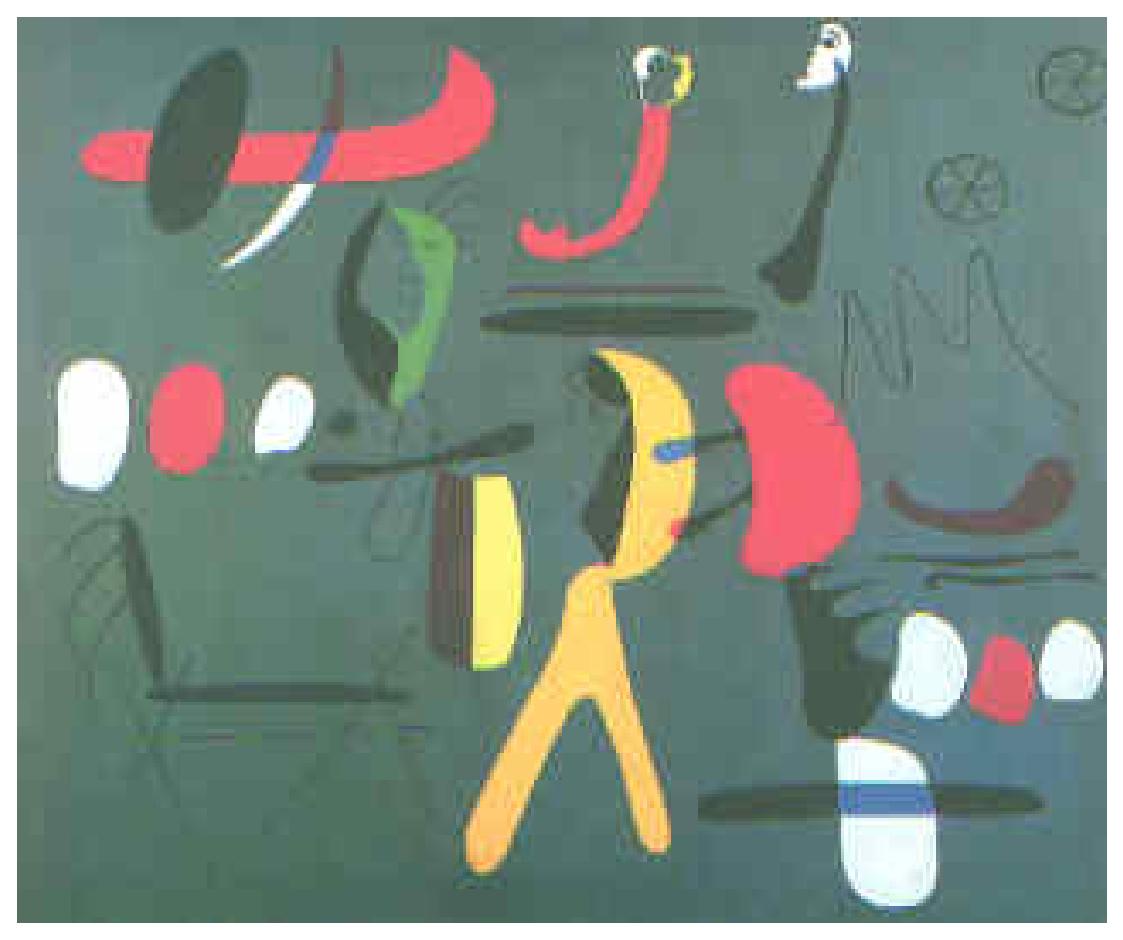
\includegraphics[width=5in]{../fig/pincolla.ps}
  \fi
  \bigskip 
  For more paintings, see {\tt http://www.bcn.fjmiro.es/}
\end{center}

\pagestyle{headings}

\newpage
\tableofcontents

%% =============================================================================

\chapter{Introduction}

\section{The \miro Group}

The \miro developers are (in alphabetical order): 
\begin{itemize}
  \item Stefan Enderle
  \item Gerhard Kraetzschmar
  \item Stefan Sablatn�g
  \item Steffen Simon
  \item Hans Utz
\end{itemize}

%% =============================================================================

\chapter{Requirements}

\begin{itemize}
  \item The Linux-kernel must be compiled with multicast enabled.
  \item ACE 5.2.x and TAO 1.2.x (we currently recommend the latest beta)
  \item gcc 2.95.3 (and above)
  \item QT 2.3 (and above)
  \item doxygen / LaTeX (for documentation)
  \item {\tt /soft/ACE\_wrappers/ace} must be part of {\tt LD\_LIBRARY\_PATH}
\end{itemize}

%% =============================================================================

\chapter{Directory Structure}

\begin{verbatim}
Miro
  |
  +--- idl                        all idl descriptions
  +--- include                    includes (empty)
  |      |
  |      +-- make_includes        includes for make
  +--- src
  |      |
  |      +-- abus                 abus utilities
  |      +-- buttons              B21 button interface implementation
  |      +-- mcp                  mcp utilities (b21 mobile base)
  |      +-- miro                 miro class framework and auto-generated idl files
  |      +-- msp                  msp utilities (sonar, infrared tactile)
  |      +-- base                 B21 interface implementations (sonar, IR, tactile, ...)
  |      +-- b21Base              B21 base services binary
  |      +-- laser                SICK laser service
  |      +-- speech               speech service (DoubleTalk cards)
  |      +-- psos                 psos utilities
  |      +-- pioneer              Pioneer1 interface implementations (sonar, motion, ...)
  |      +-- pioneerBase          Pioneer1 base services binary
  |      +-- can                  can bus utilities
  |      +-- sparrow              Sparrow99 interface implementations (infrared, motion, ...)
  |      +-- sparrowBase          Sparrow99 base services binary
  |      +-- video                Frame grabber interface
  |      +-- image                Frame grabber interface (deprecated)
  +--- bin                        all binaries
  +--- tests                      test suite
  +--- performance-tests          test suite for service/hardware performance
  +--- examples                   set of examples
  +--- utils                       
  |      |
  |      +-- qtRangeSensor        GUI range sensor visualization
  |      +-- qtTouchPad           GUI remote motion control by mouse
  |      +-- qtJoyStick           GUI remote motion control by joystick
  |      +-- notify               generic logging utilities
  |      +-- policyEditor         GUI PolicyEditor for behaviour programming
  |      +-- logPlayer            GUI player for log files
  |      +-- nsIOR                CORBA Naming Service IOR retrival utility
  |      +-- sparrow              Sparrow99 utilities
  |      +-- makeParams           Parameter file auto code generation (soon to come)
  +--- doc
  |      |
  |      +-- html                 html documentation (doxygen)
  |      |     |
  |      |     +-- idl (*)        documentation of idl interfaces (index.html)
  |      |     +-- cpp (*)        documentation of c++ class framework
  |      +-- tex                  TeX documentation (miro_manual.ps, miro_reference.ps)
  +--- lib                        all libraries
\end{verbatim}

Note: \\ 
The directories marked with {\tt (*)} are not part of the \miro
repository but are dynamically built when calling
{\tt make}.

%% =============================================================================

\chapter{Make}

The following targets can be called in the main Makefile:
\begin{itemize}
  \item all (default)
  \item depend (dont call before first complete build!)
  \item clean (remove object files)
  \item distclean (remove all generated files)
\end{itemize}

Simply typing {\tt make} calls the target {\em all}.  To get the
documentation built, change into the directory \$(MIRO\_ROOT)/doc and
call make. Note that doxygen has to be installed.

%% =============================================================================

\chapter{Styleguide}
%% styleguide.tex

\section{Files}


\subsection{Header Files vs.\ Source Files}

\begin{description}
\item[Header files:]
  These files contain the {\em declarations} of
  classes, functions, and constants that must be known to use the code. Header
  files must not contain function bodies, methods, and variable
  definitions. This is important, because each header file is included in
  all source files that need the declarations and so it may only contain
  declarations that may be duplicated.
\item[Source files:]
  These files contain the {\em definitions} of
  methods, functions, and variables.
\end{description}

Exceptions: 

\begin{description}
\item[Inline code:]
  Methods and functions that are very small or
  mainly used in loops are often implemented as inline code. The function is
  not called, but the function body is directly substituted in
  the code.
\item[Template definitions:]
  These are generic class or function
  definitions, eg.\ a generic vector. The exact type (eg.\ vector of strings)
  is given at compile time. Template are mostly used in general class
  libraries.
\end{description}

Both exceptions must be known at compile time. This means that they can not be
implemented in a source file ({\tt .c}-file), then compiled to an object
file, and later linked to the application. In order to make it explicit that
the header file contains code, inline code and template definitions are
written into separate header files ({\tt .ih} and {\tt .th}). These
files are included by the standard header file ({\tt .hh}, see section
\ref{SEC_FILE_STRUCTURE} item \ref{ITEM_IH_TH} and the example in
\ref{SEC_GENERIC_HEADER}).


\subsection{File Extensions}

\begin{tabular}{ll}
  {\tt .cc}  & C++ file \\
  {\tt .c}   & C file \\
  {\tt .hh}  & C++ header file\\
  {\tt .h}   & C header file \\
\end{tabular}


\subsection{File Names}

\begin{enumerate}
\item File names begin with a lowercase letter.
\item In names which consist of more than one word the words are
  written together and each word that follows the first is begun with an
  uppercase letter. \\ 
  Example: {\tt laserClientGlobals.cc}
\item Client and server modules are implemented in files named
  {\tt moduleServer.cc/hh} and {\tt moduleClient.cc/hh}. The header
  files are included by the user. \\ 
  Example: {\tt laserClient.hh}, {\tt sonarClient.hh}
\item Internal files used by a client or server module are named
  {\tt moduleServerSubfile.cc/hh} or {\tt moduleClientSubfile.cc/hh}.
  These header files are not included by the user. \\
  Example: {\tt laserClientGlobals.hh}, {\tt laserClientTypedefs.hh}
\end{enumerate}


\subsection{File Structure}
\label{SEC_FILE_STRUCTURE}

\begin{enumerate}
\item In C files, {\tt \#ifdef c\_plus\_plus extern "C"} must be
  used in order to compile the files with a C++ compiler. \\
  Remark: See the example in \ref{SEC_GENERIC_HEADER}. \\
  {\em Not implemented yet !!    Exact implementation !!}
\item The directive {\tt \#include "filename.hh"} is used for
  user-prepared include files.
\item The directive {\tt \#include <filename.hh>} is used for
  include files from libraries.
\item To avoid multiple includes of files, each header file must
  define the constant {\tt \_FILENAME\_H} and contain an
  {\tt \#ifndef/\#define} block at the beginning and an
  {\tt \#endif} at the end of the file. \\
  Remark: See the example in \ref{SEC_GENERIC_HEADER}. 
\end{enumerate}


\subsubsection{Generic Header File}
\label{SEC_GENERIC_HEADER}

\lstinputlisting[frame=tb]{Generic_header.cpp}

%% -----------------------------------------------------------------------------

\section{Identifier Names}
\label{SEC_IDENT_NAMES}

\begin{enumerate}
\item Classes begin with an uppercase letter. \\
  Example: {\tt LaserScan, Vector}
\item Methods, functions, objects (instances), and variables begin
  with a lowercase letter. \\ 
  Example: {\tt write(..), sonar.get(..), int number}
\item Pointer variables have the prefix {\tt p}. \\
  Example: {\tt Laser* pLaser;}
\item \label{ITEM_NAME_CONVENTION} 
  In names which consist of more than one word the words are
  written together and each word that follows the first is begun with an
  uppercase letter. \\ 
  Example: {\tt sonarScanVector}
\item Do not use underscores to begin identifiers. \\
  Remark: Underscores at the beginning are often used by internal compiler
  variables. One should be able to distinguish them easily from user variables.
\item Do not use underscores to separate words in identifiers. \\
  Exception: Item \ref{ITEM_UPPERCASE_CONSTANTS}.
\item \label{ITEM_UPPERCASE_CONSTANTS} Constants are written in
  uppercase letters where underscores are used to separate words. \\ 
  Example: {\tt VECTOR\_LENGTH, PI\_TIMES\_PI} \\
  Remark: See section \ref{SEC_GENERAL} item \ref{ITEM_NO_DEFINES} for the use
  of constants.
\item Names must differ by more than only the use of uppercase and
  lowercase letters.
\end{enumerate}

%% -----------------------------------------------------------------------------

\section{General}
\label{SEC_GENERAL}

\begin{enumerate}
\item In {\tt \#include} statements, absolute path names must not be used. \\
  Remark: Use compiler option {\tt -I} to specify include paths.
\item In {\tt \#include} statements, relative path names should not be used. \\
  Remark: Use compiler option {\tt -I} to specify include paths.
\item \label{ITEM_NO_DEFINES} Constants should not be defined with
  {\tt \#define}. Use the directive {\tt const} instead to indicate
  constants whenever possible. \\ 
  Example: {\tt const int VECTOR\_LENGTH = 20;} \\ 
  {\em Not:} {\tt \#define VECTOR\_LENGTH 20} \\ 
  Remark: This allows strict type checking by the compiler.
\item \label{ITEM_NO_MACROS} Do not use macros ({\tt \#define}.) \\
  Remark: Use inline functions for fast computation and templates functions for
  genericity.
\item Each function should contain a header explaining the
  functionality, the parameters, and the return value.
\item If data structures are passed as parameters to functions,
  references should be used instead of pointers. \\ 
  Example: {\tt void writeLaserScan(LaserScan\& laserScan);} \\
  {\em Not:} {\tt void writeLaserScan(LaserScan* pLaserScan);} 
\item The keyword {\tt const} has to be used to indicate that
  parameters are not changed. \\ 
  Example: {\tt void writeLaserScan(const LaserScan\& laserScan);} \\
  {\em Not:} {\tt void writeLaserScan(LaserScan\& laserScan);}
\item Names of objects should contain the class name. \\
  Example: {\tt LaserScan laserScan;} \\
  {\em Not:} {\tt LaserScan scan;} 
\end{enumerate}



%%% Local Variables: 
%%% mode: latex
%%% TeX-master: "servers"
%%% End: 


%% =============================================================================

\chapter{Source Code Documentation}

doxygen is used

Example:

\begin{lstlisting}[frame=tb]{}
//! Brief online description of the class
/**
 * Some comments about this class are written here.
 * You can use multiple lines.
 *
 * An empty line produces a new paragraph.
 *      
 * @author Stefan Enderle  (an author can be given!)
 */
class MyClass : public some other class
{
private:
  /**
   *  say something about this variable
   */
  double d;

public:
  /**
   *  say something about this method 
   *
   * @exception SOME_EXCEPTION                    
   *
   * @param a This param is used for something nice
   */
  bool method(int a);
};
\end{lstlisting}

%% =============================================================================

\input{refman}

%% !!! Be sure, that no other stuff comes here. particularly no \end{document}

%\chapter{Class Reference}
%\label{SEC_CLASS_REFERENCE}
%\input{miro_class_reference.nh}
%\input{miro_idl_reference.nh}
%\printindex
%\end{document}




